
\capitulo{3}{Conceptos teóricos}

Este punto nace ante la necesidad de enmarcar el proyecto dentro de las tecnologías y elementos que utilizaremos durante todo el proyecto y que no tienen por qué conocerse.

El término ‘domótica’ es el pilar principal del proyecto y, por ello, comenzaré explicando lo que es y cómo lo enfocaremos:

\section{Domótica}
La domótica podemos definirla como aquel conjunto de elementos capaces de automatizar una vivienda aportando un beneficio.
En nuestro caso, nuestro sistema domótico deberá controlar luces, persianas y calefacción permitiendo un aumento del confort y la seguridad, además de permitir un consumo eficiente de recursos a la hora de climatizar la vivienda.

\section{GPIO}
Éstos son unos puertos de entrada y salida conformados en forma de pines que están albergados en las placas Raspberry Pi\cite{misc:RbPWeb}. Con ellos enviaremos órdenes a otros dispositivos externos para que realicen las tareas que les designemos. En nuestro caso, servirán para controlar unos relés para conseguir una acción final.

\section{API}
Es el acrónimo de ‘Application Programming Interfaces’ que, traducido al castellano significa ‘Interfaz de Programación de Aplicaciones’. Estas interfaces nos sirven información que podremos utilizar en un desarrollo.
Por ejemplo, para obtener la ubicación de la máquina Raspberry Pi accedemos a una API pública que nos devolverá información que podremos procesar a nuestro gusto.
Podemos acceder a una URL como esta  \url{http://ip-api.com/json/?fields=country,regionName,city,lat,lon,isp,query} y obtendremos los valores de país, región, ciudad, latitud, longitud, ISP y dirección IP.
Estos valores, podremos recogerlos con beautifulsoup\footnote{Beautifulsoup es una librería de Python para hacer web scraping} y procesarlos desde Python como json.

\section{Json}{json\cite{misc:Json}}
Es el acrónimo en inglés de ‘JavaScript Object Notation’ y sirve para almacenar información de forma estructurada mediante etiquetas <<key>> y etiquetas <<value>> del siguiente modo: : \\
\{\\``country'':``Spain'',\\ ``regionName'':``Madrid'',\\ ``city'':``Getafe'',\\\}\\

En ella, podemos ver que las etiquetas <<key>> son las que están a la izquierda de los dos puntos y las etiquetas de la derecha son las <<value>>.

\section{RETB}
Es el acrónimo de Reglamento electrotécnico para baja tensión y en él se recoge la normativa eléctrica aplicable en domicilios.
Esta norma acaba de ser actualizada y podemos disponer de la información en páginas oficiales como puede ser el BOE\cite{manual:REBT}.
Del documento ICT-BT-21\cite{manual:ICT-BT-21} podemos extraer información para realizar las instalaciones eléctricas de nuestro sistema domótico como el número máximo de cables a introducir por un tubo eléctrico.

\section{Normativa de ICT}
Como figura en el \textit{BOE 143, de 16 de junio de 2011, El Reglamento regulador de las infraestructuras comunes de telecomunicaciones para el acceso a los servicios de telecomunicación en el interior de las edificaciones, aprobado por el Real Decreto 346/2011, de 11 de marzo}:
Debemos regirnos por esta normativa a la hora de hacer cualquier instalación de comunicaciones nueva dentro de domicilios.
Podemos informarnos y ampliar información en la publicación en la sección de ICT en el BOE\cite{manual:ICT}.

Por otro lado, disponemos de guías para instaladores con dibujos y tablas que facilitan la comprensión, como puede ser la documentación que publica Televés\cite{manual:ICT-Televes}.

De este punto, obtendremos la norma para introducir cableado ICT\cite{manual:ICT} conforme a norma.

Tras hacer un estudio en mi domicilio, no necesitaré utilizar la normativa de ICT\cite{manual:ICT} porque toda la instalación se realizará mediante canales eléctricos, pero está bien conocer la norma para, en caso de necesitarla, poder hacer uso de ella correctamente.

\section{Cableado estructurado}
El establecimiento de un sistema de cableado estructurado consiste en la organización de los cables en un recinto conforme a una norma y constituye el nivel básico de cualquier red de comunicaciones.
Al contar y cumplir con este estándar nos damos cuenta de que tendremos instalaciones limpias, uniformes, seguras y escalables, facilitando la supervisión, el mantenimiento y posibles migraciones de tecnologías.
Un sistema de cableado genérico dispone de tres subsistemas, Troncal, de Edificio y Horizontal. En nuestro proyecto únicamente trataremos con el subsistema horizontal.

En este proyecto no contaremos con un gran número de cables, pero no está de más realizar una instalación lo más correctamente posible con unas normas de referencia

\section{WiFi}
Es una tecnología de comunicaciones de forma inalámbrica o “Wireless”. WiFi\footnote{Traducción del inglés: 'Wireless Fidelity'} es el acrónimo traducido de “Fidelidad Inalámbrica”.
Estas tecnologías inalámbricas se rigen por la norma \underline{IEEE 802.11}\cite{manual:IEEE802.11}.
En la web oficial del organismo podremos comprobar qué estándares dentro del 802.11 están vigentes y cuáles no.

\section{UTP}
Es un tipo de cableado de datos que se compone de 4 pares de cables sin apantallar que están albergados dentro de una camisa de PVC, ver imagen~\ref{Img:Bobina UTP}

\begin{figure}
    \centering
    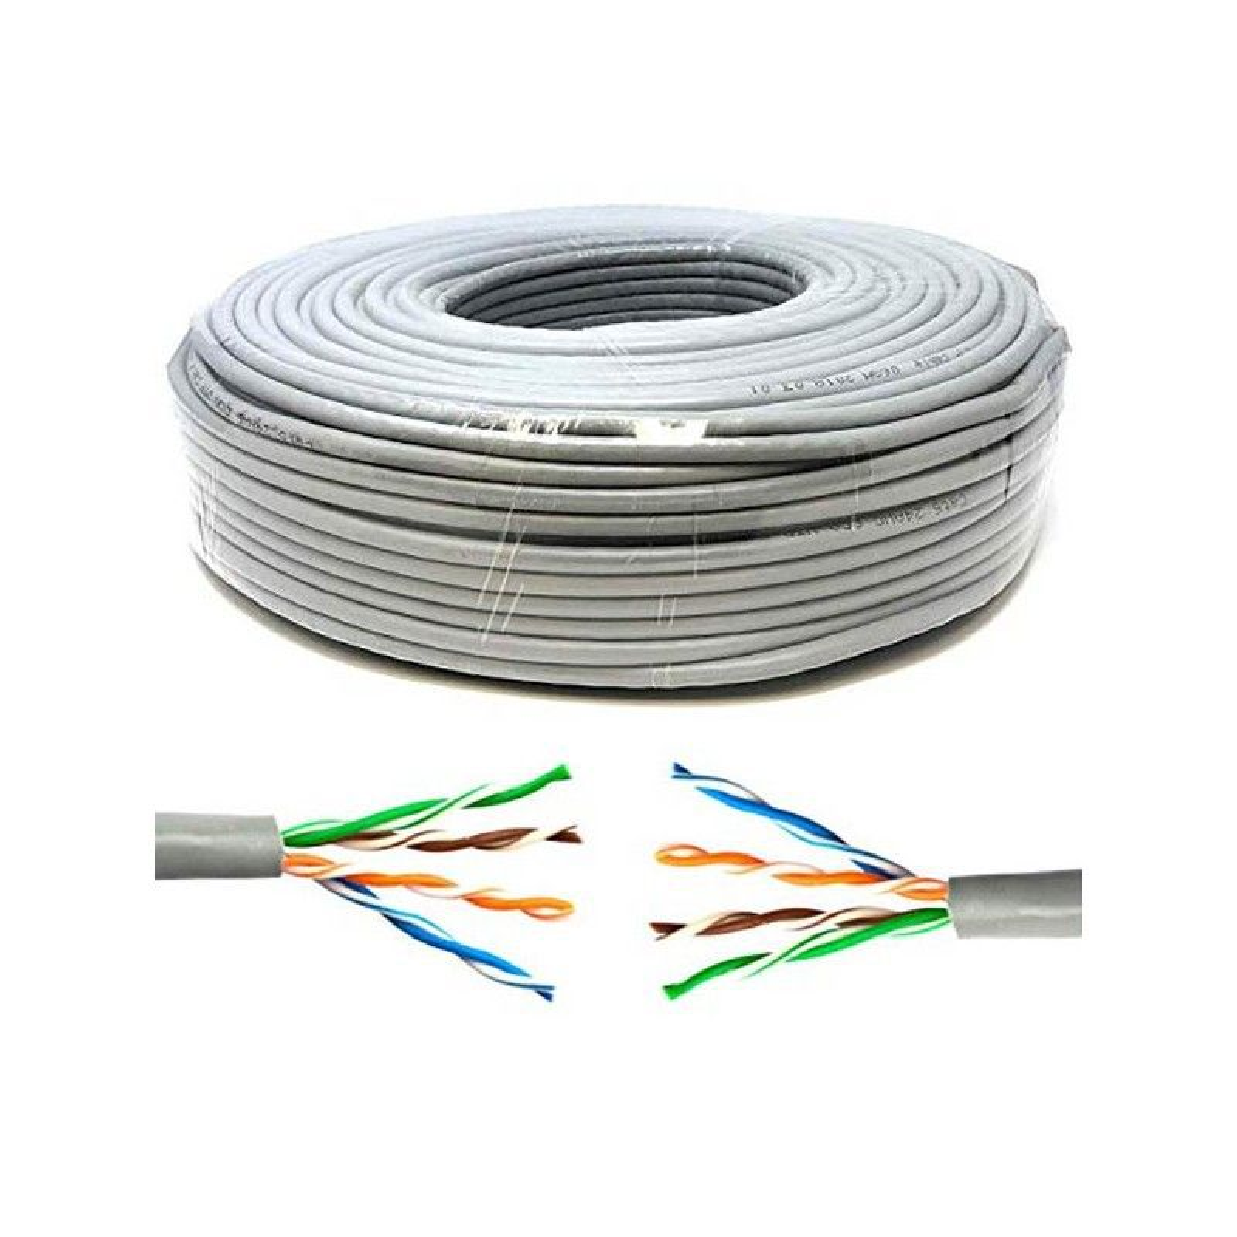
\includegraphics[width=.6\textwidth]{img/bobina_UTP.pdf}
    \caption[Bobina UTP]{Bobina UTP con muestra del mismo con corte de camisa exterior. Imagen de \url{https://solarmat.es}\cite{wiki:Creative}. \url{https://cr.eativecommons.org/licenses/by-sa/3.0/deed.es_ES} } \label{Img:Bobina UTP}
\end{figure}

Existen diferentes tipos de cables de datos: UTP, STP, FTP:
\begin{itemize}
\item Los cables \textbf{UTP} (del ingles <<Unshielded Twisted Pair>> o <<Par trenzado no apantallado>>) no disponen de protección ante interferencias electromagnéticas. Ver imagen ~\ref{Img:Muestra UTP}.

\begin{figure}
    \centering
    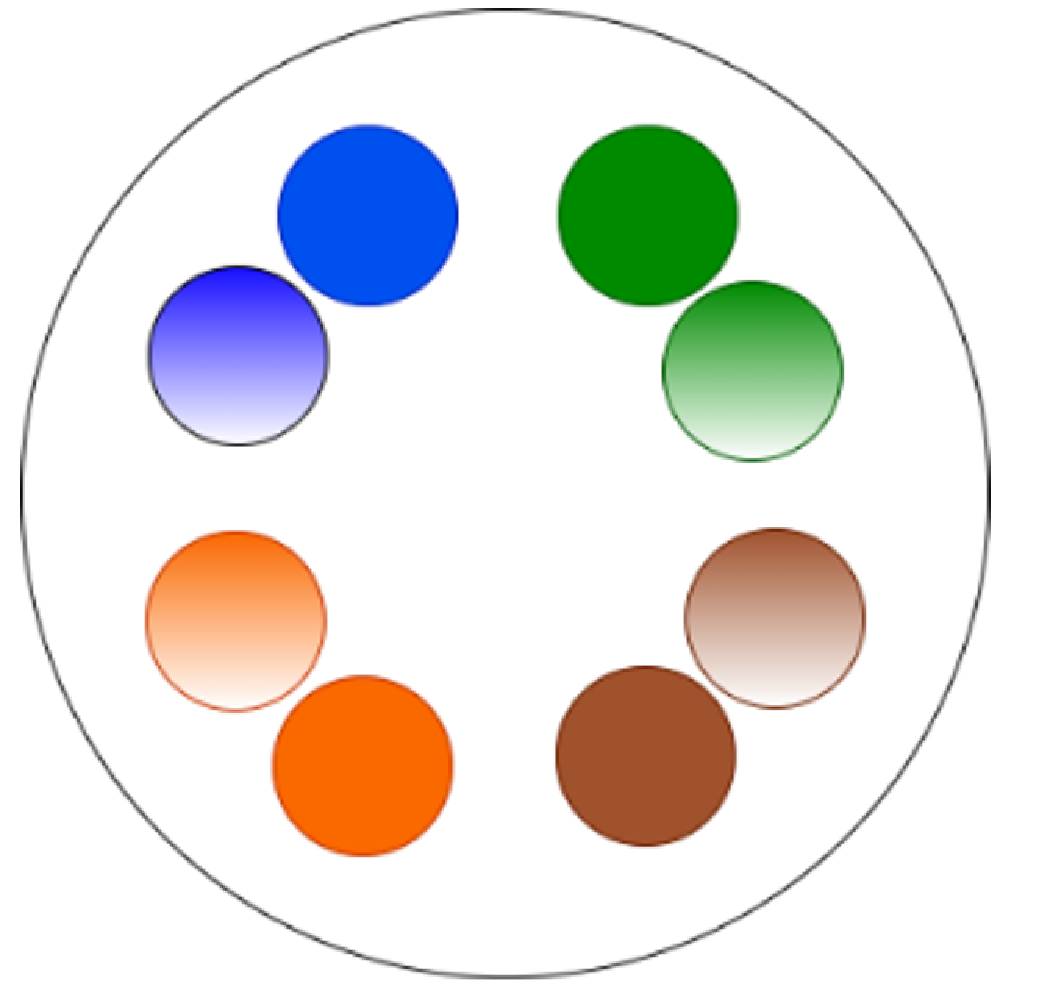
\includegraphics[width=0.4\textwidth]{img/UTP.pdf}
    \caption{Diagrama de muestra de cable UTP} \label{Img:Muestra UTP}
\end{figure}

\item Los cables \textbf{FTP}(del inglés <<Foiled Twisted Pair>> o <<Par trenzado con pantalla global>>) disponen de una pantalla global contra interferencias electromagnéticas dentro de la camisa de PVC que recoge los 4 pares destinados a transmisión de datos. Ver imagen ~\ref{Img:Muestra FTP}.

\begin{figure}
    \centering
    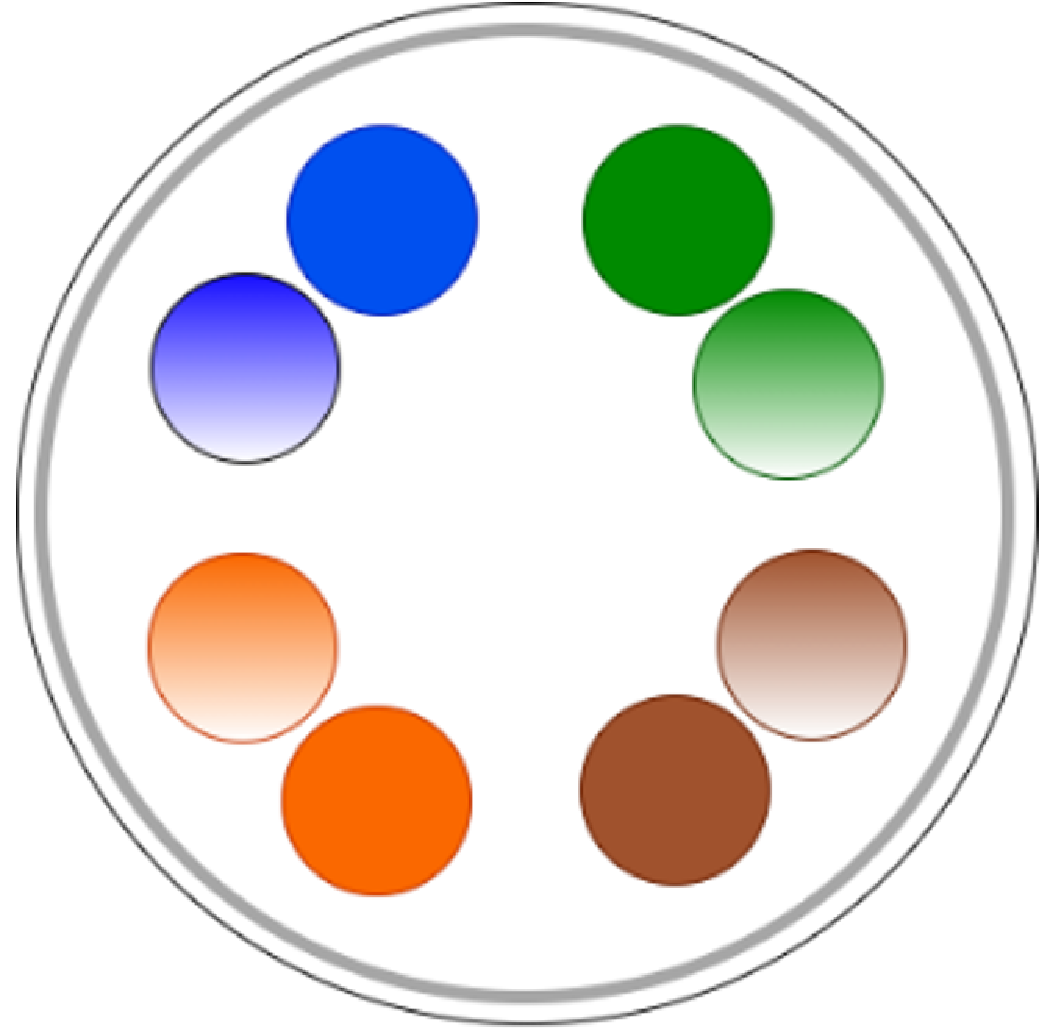
\includegraphics[width=0.4\textwidth]{img/FTP.pdf}
    \caption[Diagrama de muestra de cable FTP]{Diagrama de muestra de cable FTP. Podemos observar la camisa exterior del cable} \label{Img:Muestra FTP}
\end{figure}

\item Los cables \textbf{STP}(del inglés <<Shielded Twisted Pair>> o <<Par trenzado apantallado>>) disponen de una pantalla contra interferencias electromagnéticas por cada par de cables pero, además, también cuentan con una malla metálica exterior. Ver imagen ~\ref{Img:Muestra STP}.
\begin{figure}
    \centering
    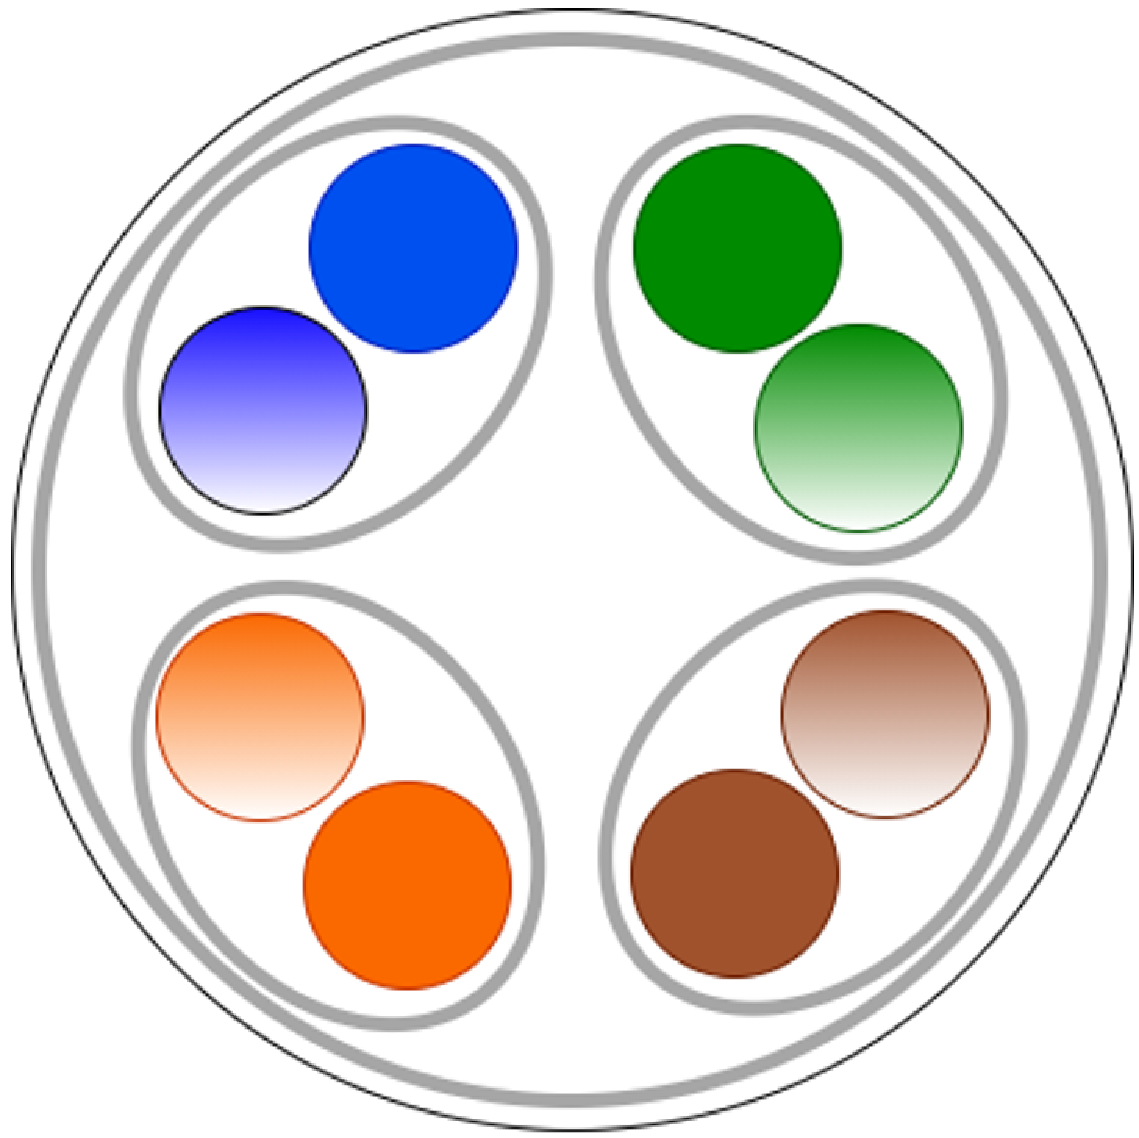
\includegraphics[width=0.4\textwidth]{img/STP.pdf}
    \caption[Diagrama de muestra de cable STP]{Diagrama de muestra de cable STP. Vemos camisa exterior y por pares} \label{Img:Muestra STP}
\end{figure}

En nuestro caso utilizaremos UTP puesto que no necesitamos un apantallamiento ya que no transmitiremos datos y tampoco tendremos un alto grado de interferencias.

\end{itemize}

